\documentclass{polytech/polytech}

\typereport{stagedi5}

\reportyear{2017-2018}
\title{Réalisation d'un outil de cartographie sur le progiciel Amplitude}
\student{Romain}{ROUSSEAU}{romain.rousseau@etu.univ-tours.fr}
\academicsupervisor{Yannick}{KERGOSIEN}{yannick.kergosien@univ-tours.fr}
\industrialsupervisor[Responsable Cellule Architecture]{Alexandre}{DURAND}{alexandre.durand@soprabanking.com}

\company[images/logoSopra]{Sopra Banking}{47 rue Christiaan Huygens \\ 37073 Tours Cedex 2 - France}{www.soprabanking.com}

\resume{}

\motcle{}

\abstract{}

\keyword{}


%%%%%%%%%%%%%%%%%%%%%%%%%%%%%%%%%%%%%%%%%%%%%%%%%%%%%%%%%%%%%%%%%%%%%%%%%%%%%%%%%%%%%%%%%%%%%%%%%%%
%%%%%%%%%%%%%%%%%%%%%%%%%%%%%%%%%%%%%%%%%%%%%%%%%%%%%%%%%%%%%%%%%%%%%%%%%%%%%%%%%%%%%%%%%%%%%%%%%%%

\begin{document}

\chapter*{Introduction}


Ce rapport présente mon stage d'assistant ingénieur réalisé dans l'entreprise \textit{Sopra Banking Software} à Tours. Le sujet du stage était la réalisation d'un outil de cartographie pour le progiciel nommé \textit{Amplitude} de l'entreprise. Le stage a débuté le 9 avril 2018 avant de s'achever le 31 août de la même année.

Le stage de cinquième année a pour but d'appliquer les connaissances acquises lors des précédentes années d'étude. Il doit représenter une synthèse de l'ensemble des caractéristiques qu'un ingénieur doit avoir dans un environnement concret. Alors que le stage de troisième année sert à découvrir le monde de l'entreprise et que celui de quatrième année sert à faire le premier pas vers le métier d'ingénieur, le stage de dernière année permet de travailler dans une équipe installée pour mener à bien un projet, dans son intégralité ou tout du moins sa majorité selon les cas. Ce stage est censé donner une autonomie supérieure aux étudiants, qui doivent prendre des décisions et avoir la possibilité de donner leur avis sur les opérations en cours, ce qui en fait ainsi, une expérience nécessaire pour le métier. 

Il se déroule sur une période d'au minimum 18 semaines, ce qui permet de pouvoir réaliser des projets avec une envergure dont les étudiants-ingénieurs n'ont jamais eu l'occasion de faire durant leur cursus. Il s'agit du stage le plus important de la formation car il s'agit du plus complet, du plus formateur et de manière générale, du plus intéressant. Il apporte une expérience non négligeable et représente la dernière marche avec l'arrivée dans la vie active.

Le secteur de l'informatique est très porteur et les offres de stage sont donc très nombreuses et variées. L'opportunité de stage dans l'entreprise \textit{Sopra Banking Software} est venue lors du Forum des Entreprises qui se déroule à Polytech pendant le mois de novembre. J'y ai pu rencontrer de nombreux acteurs du secteur et obtenir des entretiens avec plusieurs d'entre eux, dont notamment deux à Sopra sur le site de Tours. À la suite de ces entretiens, j'ai pu faire mon choix parmi les propositions. J'ai retenu celle de la Cellule Architecture de \textit{Sopra Banking Software} pour plusieurs raisons. Tout d'abord, le domaine de la banque m'a toujours intéressé, j'ai déjà fait mon stage de 4ème année chez Worldline du côté des paiements en ligne et je voulais découvrir un autre aspect du domaine. Ensuite, j'avais envie de faire partie d'un projet que ne soit pas monotone et qui me permette d'acquérir de nouvelles connaissances sur des technologies que je ne maîtrise pas ou très peu. Et c'était le cas avec cette offre qui combinait tous les aspects d'un projet, de l'expression des besoins jusqu'au développement en passant par la modélisation ou encore le chiffrage, le tout en utilisant des technologies récentes, variées et performantes. 

Les chapitres qui vont suivre exposeront les principales phases de mon stage, en commençant d'abord par une présentation de l'entreprise et du projet en lui-même. La suite sera consacrée à mon parcours au sein de l'équipe, avec dans un premier temps, une phase de formations sur les différents éléments de l'entreprise ainsi que sur les technologies qui seront utilisées; puis, à la modélisation de l'outil, avec l'élaboration des diagrammes de Gantt, et le chiffrage du projet; et enfin le développement en lui-même. 


\part{Présentation de l'entreprise et du projet}


Cette partie sera consacrée à la présentation du cadre général de mon stage, c'est-à-dire le groupe \textit{Sopra}, sa filiale \textit{Sopra Banking Software}, le progiciel Amplitude et la présentation générale du sujet. 


\chapter{Le groupe \textit{Sopra Steria} et \textit{Sopra Banking Software}}

\section{Histoire des deux groupes: \textit{Sopra} et \textit{Steria}}

\begin{figure}
	
\includegraphics[scale=1]{images/sopralogo}
\end{figure}

\textit{Sopra Steria} est une entreprise de services du numérique qui propose des prestations de conseils, des services technologiques et qui édite des logiciels métiers dans trois principaux domaines: les ressources humaines, l'immobilier et la banque. Définie comme leader européen de la transformation numérique, l'entreprise, de par sa diversité, propose l'un des portefeuilles d'offres les plus complets du marché. L'une des principales motivations du groupe est d'accompagner ses clients dans leur transformation numérique et les aider à faire le meilleur usage de leurs outils. Parmi les actuels clients de l'entreprise, on peut citer des grands noms comme Airbus, La Banque Postale, le Ministère de la Défense, EDF, le Ministère des Finances, la SNCF, Easyjet, et bien d'autres.  

Comme beaucoup de SSII à grandes envergures, \textit{Sopra Steria} est le fruit de nombreuses acquisitions et fusions au fil du temps. Tout d'abord, \textit{Sopra} et \textit{Steria} composaient deux entreprises distinctes. Elles ont toutes les deux été créées à la fin des années 70 (en 1968 pour \textit{Sopra} et en \textit{1968} pour \textit{Steria}). Les deux entreprises se développent dans les années qui suivent. \textit{Sopra} (acronyme pour \textbf{SO}ciété de \textbf{PR}ogrammation et d'\textbf{A}nalyses) investit dans le développement de logiciels, notamment dans le domaine bancaire et les ressources humaines. Le groupe \textit{Sopra} fera son entrée à la bourse de Paris en 1990 après avoir travaillé sur un projet avec Ministère de l'Intérieur. De son côté, \textit{Steria} (acronyme de Société d'étude et de réalisation en informatique et automatisme) réalise de grandes signatures du côté de la sphère publique, en informatisant l'AFP en 1975 ou encore en participant au développement du Minitel en 1981 par exemple. 

Le milieu des années 90 marque le début d'une série d'acquisitions de la part des deux groupes. \textit{Sopra} s'implante au Royaume-Uni, en Espagne, en Italie et en Allemagne en 1999 tandis que \textit{Steria} rentre à la bourse de Paris cette même année. Par la suite, le groupe double de taille en intégrant les activités européennes de \textit{Bull} en 2001 et se renforce dans le conseil en acquérant l'entreprise allemande \textit{Mummert Consulting} en 2005. \textit{Steria} développera considérablement ses parts de marché dans le secteur public au Royaume-Uni en acquérant la société \textit{Xansa}, expert dans le \textit{Business Output Processing}. Le groupe \textit{Sopra} quant à lui, consolide son expansion européen en créant la filiale \textit{Axway Software} en 2001 qui deviendra indépendante en 2011. En parallèle, \textit{Sopra} acquiert 100\% du groupe \textit{Delta Informatique}, société indépendante éditrice d'une offre de solutions « Global Banking » destinée aux banques de détail en France et à l’international. Suite à ce rachat et à celui d'autres sociétés et filiales, en 2012, le groupe \textit{Sopra}, reconnu pour son expertise dans les services financiers, crée la filiale \textit{Sopra Banking Software}. Les solutions dédiées aux ressources humaines feront parties d'une autre filiale appelée, \textit{Sopra HR Software}.

\section{Fusion des deux groupes et création de \textit{Sopra Steria}}


L'année 2014 marquera le rapprochement amical des deux entités. L'OPE du groupe \textit{Sopra} visant la totalité des actions de \textit{Steria} sera un succès. \textit{Sopra Group} devient ainsi \textit{Sopra Steria Group}. Le changement sera effectif le 31 décembre 2014. Suite au plan d'intégration construit conjointement par les équipes des deux entités précédentes, le groupe continue de mener sa politique basée l'acquisition de nouvelles entreprises comme \textit{Cassiopae}, éditeur spécialisé dans les solutions de crédits à l'entreprise et la gestion immobilière locative, \textit{Kentor}, société scandinave spécialisée dans le conseil, l'intégration de systèmes et la maintenance applicative, ou encore \textit{Galitt}, éditeur de solutions sur le marché des systèmes de paiement et des transactions sécurisées.

Le développement continuel du groupe lui permet d'atteindre une place importante parmi les entreprises de services numériques mondiales. Aujourd'hui, le groupe compte plus de 42 000 collaborateurs dans plus de 20 pays à travers le monde et un chiffre d'affaires de 3,8 milliards d'euros en 2017.

\section{La filiale \textit{Sopra Banking Software}}

\begin{figure}
	
\includegraphics[scale=1]{images/logoSopra}
\end{figure}

La filiale \textit{Sopra Banking Software} est un fournisseur de solutions globales comprenant, outre sa gamme de progiciels, les services d'intégration, de support et de conseil associés. Elle a été initiée suite au rachat de plusieurs entreprises du secteur bancaire dont notamment \textit{Delta Informatique} en 2011. Par ailleurs, le site \textit{Sopra Banking Software} de Tours où j'ai réalisé mon stage était auparavant un site \textit{Delta Informatique}.

Ses solutions accompagnent près de 800 banques dans 70 pays. Son objectif est d'accompagner les établissements dans leur développement et dans leur stratégie internationale, par une approche de partenariat à long terme. La société s'appuie pour cela sur l'engagement et l'expertise de plus de 3 500 personnes. Les principales zones d'activités de \textit{Sopra Banking} sont en Europe, en Afrique et au Moyen-Orient. La filiale compte un panel d'offres variées pour les clients. Parmi ces offres, on trouve notamment le progiciel \textit{Amplitude} sur lequel mon stage va se baser. 


\chapter{Le progiciel Amplitude}

\section{Présentation}

\textit{Amplitude}, de son nom complet \textit{Sopra Banking Amplitude}, est la solution de \textit{core banking} proposé par \textit{Sopra Banking Software} pour traiter de manière intégrée toutes les problématiques bancaires. Le progiciel a été développé au sein du groupe \textit{Delta Informatique} avant son acquisition par \textit{Sopra}. \textit{Amplitude} est adoptée par 200 banques dans 50 pays et s’adresse à tous types d’institutions financières, de la banque en création aux grands groupes.

Parmi les avantages listées sur le site de \textit{Sopra Banking}, on retrouve: 

\begin{itemize}
	\item Une large couverture avec plus de 80 modules métiers
	\item Un système entièrement digital ready et sécurisé
	\item Une solution évolutive et agile
	\item Une architecture orientée client et process	
\end{itemize}

Les premières mises en production d'\textit{Amplitude} datent du début des années 90. Le progiciel est basé sur le langage de programmation \textit{Informix-4GL}. Il s'agit d'un langage propriétaire développé par la société \textit{Informix} au milieu des années 80. Le langage appartient aujourd'hui à \textit{IBM} depuis le rachat d'\textit{Informix} en 2005. 


\section{Architecture générale}


Tout \textit{Amplitude}

Arborescence


\chapter{Présentation du projet}

Cartographie / Expression des besoins


\part{Tutoriels et formations}


Cette partie sera consacrée aux différents tutoriels et formations que j'ai effectué lors des premières semaines de stage (approximativement les 3 semaines du mois d'Avril). Après avoir pris connaissance du sujet et des locaux, une phase de mise à niveau sur les outils que nous allions utiliser s'imposait. Le principe était de réaliser des tutoriels préconisés par mon encadrant (tutoriels internes à \textit{Sopra} ou sur Internet) et de réaliser des comptes-rendus (ou \textit{Proof of Concept}) sur les outils observés pour que les personnes souhaitant s'intéresser au sujet puissent avoir un support disponible. Les formations étaient portées sur trois technologies principales : \textit{Spring Boot}, \textit{Spring Data} et \textit{Angular}. Ces technologies seront détaillées dans cette partie.

Avant de rentrer dans les détails, il est important d'avoir quelques connaissances en développement au préalable, en particulier en langage Java, sur certains frameworks et sur l'outil de construction de projet \textit{Maven}. Les notions basiques de \textit{Maven} sont résumées rapidement sur le site de documentation d'Apache ici : \url{https://maven.apache.org/guides/getting-started/maven-in-five-minutes.html}.


\chapter{Spring Boot}


\textit{Spring Boot} a pour but de faciliter la création d'application utilisant \textit{Spring} en automatisant ses configurations. \textit{Spring Boot} permet par ailleurs de créer pour un projet, un exécutable unique contenant toutes les dépendances nécessaires. Les objectifs annoncés par la documentation de \textit{Spring Boot} sont les suivants : 

\begin{itemize}
	\item Proposer des solutions rapides et accessibles pour les développements \textit{Spring} ;
	\item Faciliter les configurations, même lorsque les paramètres souhaités diffèrent de ceux utilisés par défaut ;
	\item Proposer une panoplie d'options non-fonctionnelles (comme des serveurs embarqués \textit{Tomcat}, des options de sécurité, de mesures de performances, etc.) ;
	\item Aucune génération de code ni de configuration XML. 
\end{itemize}

\textit{Spring Boot} ne génère pas de code ni ne modifie les fichiers du projet. Au démarrage de l'application, \textit{Spring Boot} va dynamiquement « brancher » les composants et les configurations nécessaires au contexte du projet. Les deux principales modifications à opérer pour faire fonctionner \textit{Spring Boot} se passent sur le fichier \textit{Maven} et au travers d’annotations du framework \textit{Spring} sur les composants en action. Le détail du fonctionnement sera détaillé dans les prochaines sections. 

\textit{Spring Boot} fonctionne avec les versions Java 1.8 et supérieur. Les différentes versions des composants utilisés par \textit{Spring Boot} sont détaillés dans le guide de référence à l’adresse suivante : \url{https://docs.spring.io/spring-boot/docs/2.0.1.RELEASE/reference/htmlsingle/}.


\section{Création d'un projet avec \textit{Spring Initializr}}

Il est possible de générer un projet \textit{Spring Boot} avec toutes les dépendances que l’on souhaite \textit{Spring Initializr} à l’adresse : \url{https://start.spring.io/}. Un aperçu du site est visible sur la \autoref{fig:initializr}.

\begin{figure}
	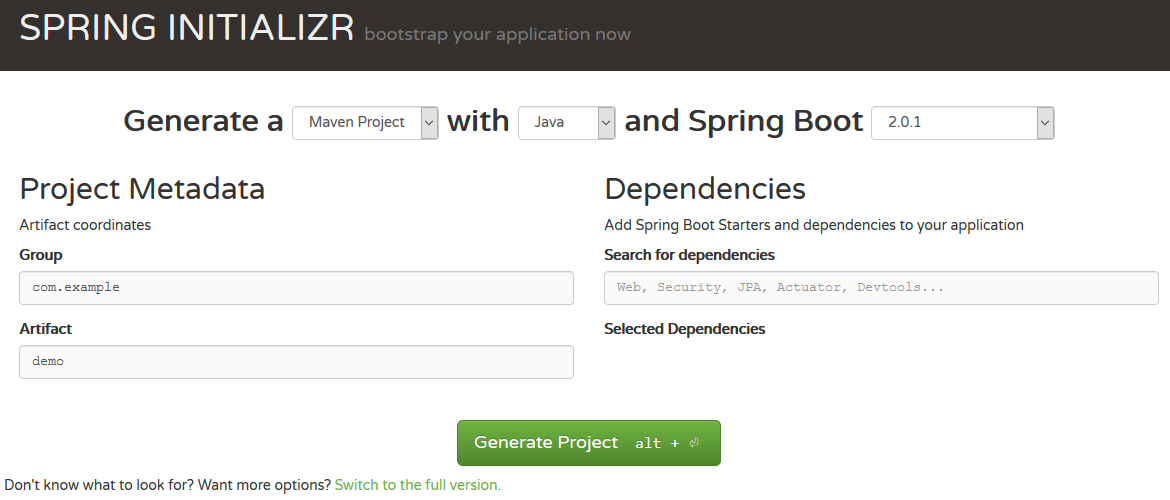
\includegraphics[scale=0.5]{images/springInitializr}
	\caption{Aperçu du site \textit{Spring Initializr}}
	\label{fig:initializr}
\end{figure}

Pour générer un projet, il suffit d’indiquer les propriétés du projet et les dépendances que l’on souhait ajouter et un modèle de projet \textit{Spring Boot} sera disponible au téléchargement. Les détails et le fonctionnement du fichier \textit{pom.xml} généré sont détaillés dans la prochaine section. 

La création d'un projet par ce biais n'est pas obligatoire, cependant dans les cas où l'on connaît par avance les principales dépendances de notre projet, cela s'avère être un gain de temps non négligeable. Le projet généré est sous forme de dossier compressé \textit{.zip} contenant la structure du projet, le fichier de construction du projet \textit{pom.xml} de \textit{Maven} avec toutes les dépendances, et les classes principales. 


\section{Utilisation avec \textit{Maven}}
\label{sec:utilisationMaven}


Pour utiliser \textit{Spring Boot} via l’outil \textit{Maven}, la solution la plus courante est de faire hériter son projet du \textit{spring-boot-starter-parent} qui contient les dépendances de bases de \textit{Spring Boot} en ajoutant cette partie au début du fichier \textit{pom.xml} :

\begin{figure}
	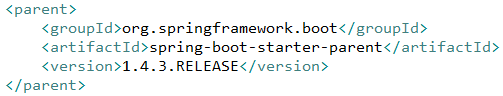
\includegraphics[scale=0.75]{images/parentSpringBoot}
	\caption{Extrait d'implémentation de la dépendance parent dans le \textit{pom.xml}}
	\label{fig:parentSpringBoot}
\end{figure}

Ensuite, dans la partie \textit{dependencies}, on ajoute les starters correspondant au type d’application que l’on souhaite réaliser. Les \textit{starters} sont des dépendances \textit{Maven} regroupant toutes les configurations voulues pour l’application.  Par exemple, si l'on souhaite réaliser une application web, on ajoute la dépendance \textit{spring-boot-starter-web} dans le fichier \textit{pom.xml}: 

\begin{figure}
	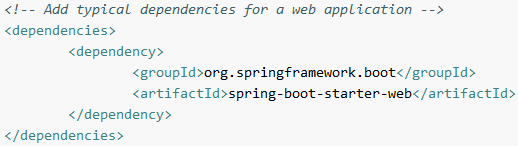
\includegraphics[scale=0.75]{images/dependencySpringBoot}
	\caption{Extrait d'implémentation d'une dépendance web dans le \textit{pom.xml}}
	\label{fig:dependencySpringBoot}
\end{figure}

Cela embarquera toutes les dépendances nécessaires au fonctionnement d'une application web, comme un serveur embarqué \textit{Tomcat} par exemple. Tous les starters suivent la même syntaxe : \textit{spring-boot-starter-*}, avec * le type de projet souhaité. Parmi les différents starters disponibles, voici un liste des plus intéressants pour plusieurs types de projets :

\begin{description}
	\item[spring-boot-starter] Starter central, auto-configure le support, le logs et les fichiers YAML.
	\item[spring-boot-starter-web] Utilisé pour réaliser des application web utilisant Spring MVC. Utilise Tomcat comme conteneur embarqué par défaut.
	\item[spring-boot-starter-thymeleaf] Utilisé pour les applications Web MVC avec les vues de Thymeleaf.
	\item[spring-boot-starter-test] Utilisé pour la réalisation de tests. Il implémente plusieurs bibliothèques de tests comme JUnit, Mockito, etc..
	\item[spring-boot-starter-actuator] Utilisé pour la mise en production, ajoute des fonctionnalités pour monitorer et gérer l’application. 
	\item[spring-boot-starter-jdbc] Utilisé pour JDBC avec le pool de connexion HikariCP.
	\item[spring-boot-starter-data-jpa] Utilisé pour Spring Data JPA avec Hibernate.
	\item[spring-boot-starter-security] Utilisé pour Spring Security.
\end{description}

La liste complète des starters se trouvent à l’adresse suivante : \url{https://docs.spring.io/spring-boot/docs/2.0.1.RELEASE/reference/htmlsingle/#using-boot-starter}.

Ensuite, pour empaqueter l'application dans un exécutable, il suffit de rajouter le plug-in maven dans la partie \textit{build} du fichier \textit{pom.xml} comme on peut le voir dans la \autoref{fig:buildSpringBoot}.

\begin{figure}
	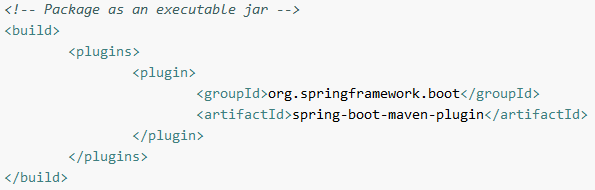
\includegraphics[scale=0.75]{images/buildSpringBoot}
	\caption{Implémentation du plug-in \textit{Maven}}
	\label{fig:buildSpringBoot}
\end{figure}

Il s’agit de l’essentiel des modifications à apporter dans le fichier de configuration de \textit{Maven} pour faire fonctionner une application \textit{Spring Boot}. Il est possible d’ajuster d’autres paramètres ou d’ajouter davantage de fonctionnalités. Par exemple, pour les applications web, la dépendance \textit{spring-boot-devtool} permet d’effectuer des rafraîchissements à la volée sans recompiler l’intégralité du code. 


\section{Éléments à ajouter dans le programme}
\label{sec:elementsSpringBoot}

La configuration des projets \textit{Spring Boot} nécessite l’utilisation d’annotations du framework \textit{Spring} pour définir l’architecture du projet et les interactions entre les composants. L’annotation principale à ajouter est \textit{@SpringBootApplication}.


Cette annotation doit être placée sur la classe principale du projet et correspond à 3 annotations \textit{Spring}:
\begin{itemize}
	\item \textit{@Configuration} qui indique que la classe est la source pour le contexte donné;
	\item \textit{@EnableAutoConfiguration} qui indique à \textit{Spring Boot} d’ajouter les configurations définies au préalable;
	\item \textit{@ComponentScan} qui indique à \textit{Spring} de regarder les configurations dans les autres classes du même package;
\end{itemize}

Ensuite, la méthode \textit{main()} utilise la fonction dédiée au lancement de l’application de \textit{Spring Boot} : \textit{SpringApplication.run()}. Sur la \autoref{fig:mainSpringBoot}, un exemple de classe principale basique utilisant la fonction \textit{run()} et l’annotation pour le lancement de \textit{Spring Boot}.

\begin{figure}
	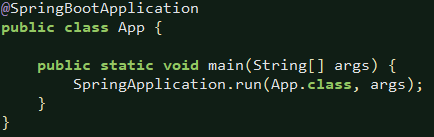
\includegraphics[scale=1]{images/mainSpringBoot}
	\caption{Fonction principale d'un projet \textit{Spring Boot}}
	\label{fig:mainSpringBoot}
\end{figure}

\textit{Spring Boot} se connecte automatiquement à la classe principale du projet. Or, il est possible qu’un projet comporte plusieurs classes principales. Pour pallier à cela, il est possible de définir la classe que l’on souhaite lancer dans le fichier \textit{pom.xml} de deux manières : soit dans la partie \textit{properties} dans une balise \textbf{<start-class>}, soit dans la partie \textit{build} dans une balise <\textbf{configuration>} comme dans la  \autoref{fig:multipleMainSpringBoot}.

\begin{figure}
	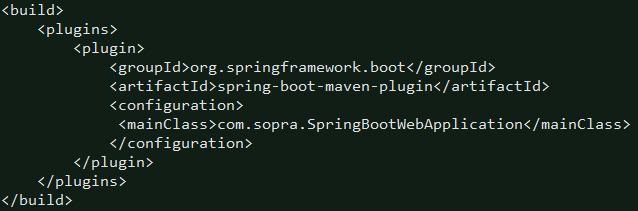
\includegraphics[scale=0.8]{images/multipleMain}
	\caption{Fichier \textit{pom.xml} en cas de multiples fonctions principales}
	\label{fig:multipleMainSpringBoot}
\end{figure}

Dans le cas où l'on souhaite réaliser des tests unitaires, on peut ajouter le starter \textit{spring-boot-starter-test} dans le fichier \textit{pom.xml}. Puis, on annote les classes de tests par \textit{@SpringBoottest} ce qui permet de notifier à \textit{Spring Boot} que la classe annotée par la balise correspond à une classe de tests et ainsi, d'ajouter les configurations automatiques nécessaires.

\section{Exemple d'application web avec \textit{Spring Boot}}

Il existe plusieurs façons de réaliser une application Web avec Spring Boot. La dépendance permettant d’importer les principales configurations est spring-boot-starter-web qui utilise Spring MVC pour fonctionner. D’autres starters peuvent être utilisés pour certains cas, par exemple pour une application web MVC, si l’on souhaite gérer les vues avec Thymeleaf ou Mustache, la dépendance spring-boot-starter-thymeleaf ou spring-boot-starter-mustache configurera automatiquement les paramètres nécessaires. 

Par défaut, Spring Boot utilise les conteneurs Tomcat. Il est possible d’utiliser un autre conteneur que Tomcat, comme Jetty par exemple, mais il faut au préalable exclure Tomcat des dépendances du fichier pom.xml, comme sur la \autoref{fig:webBuildSpringBoot}.

\begin{figure}
	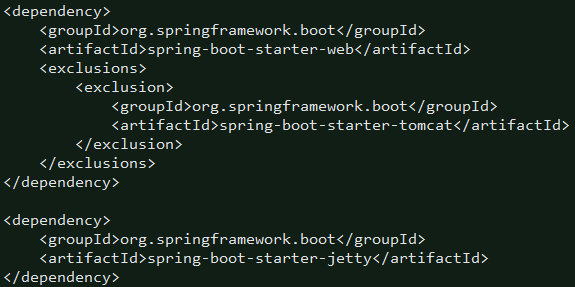
\includegraphics[scale=0.8]{images/webBuildSpringBoot}
	\caption{Fichier \textit{pom.xml} en cas de multiples fonctions principales}
	\label{fig:webBuildSpringBoot}
\end{figure}

Le port d’écoute utilisé par défaut est le 8080. Pour le modifier, plusieurs possibilités existent :

\begin{itemize}
	\item Indiquer le port souhaité dans un fichier \textit{application.properties} ou \textit{application.yml};
	\item Faire figurer dans une méthode le changement de port;
	\item Le faire figurer en ligne de commande au lancement du \textit{jar} exécutable (exemple : \javacode{java -jar -Dserver.port=8888 spring-boot-example-1.0.jar}).
\end{itemize}

Dans le cas où un port est spécifié à la fois dans le fichier \textit{application.properties} et dans le code, alors c’est le code spécifié dans le code qui sera pris en compte.

Ensuite, dans le code, il suffit d’annoter la classe main comme expliquée dans la \autoref{sec:elementsSpringBoot} et d’ajouter un contrôleur basique pour faire fonctionner le tout. 

\section{Gestion de base de données}

La gestion et la configuration d’une base de données avec Spring Boot se fait de façon simple et automatisé. Il existe plusieurs starters permettant de gérer une base de données avec Spring Boot, ici nous allons évoquer le fonctionnement avec JDBC, puis avec JPA et Spring data.

Il y a principalement 3 dépendances à ajouter dans le fichier \textit{pom.xml} si l’on souhaite utiliser JDBC: spring-boot-starter pour la configuration principale de l’application, spring-boot-starter-jdbc pour les dépendances avec JDBC et le driver de la base de données que l’on souhaite utiliser. Comme pour les autres dépendances, spring-boot-starter-jdbc utilise Tomcat pour gérer les connexions. Pour modifier cela, il faut d’abord exclure la dépendance Tomcat, puis ajouter celle que l’on souhaite par la suite. Par exemple, si l’on utilise une base de données Oracle et une connexion via DBCP2, les dépendances du fichier \textit{pom.xml} seront tels qu'on peut les trouver sur la \autoref{fig:bddBuild}. 

\begin{figure}
	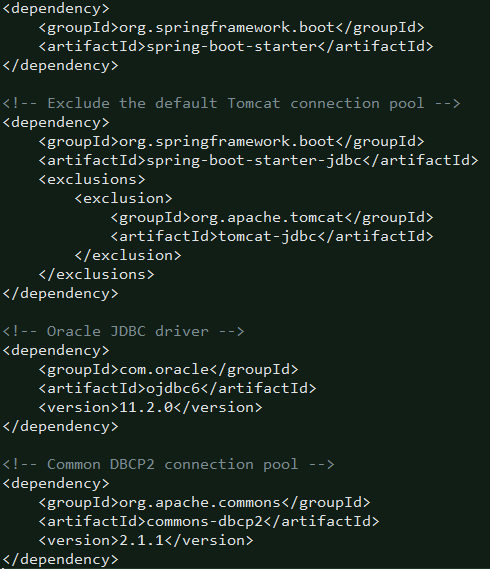
\includegraphics[scale=0.75]{images/bddPom}
	\caption{Exemple de dépendances dans le \textit{pom.xml} pour la gestion d'une base de données}
	\label{fig:bddBuild}
\end{figure}

Ensuite, les paramètres de connexions de la base de données sont indiqués dans le fichier de configuration \textit{application.properties} comme sur la \autoref{fig:bddProperties}.

\begin{figure}
	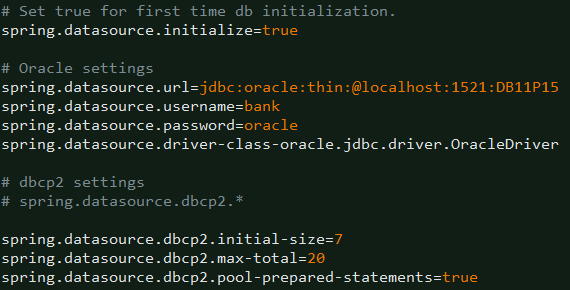
\includegraphics[scale=0.8]{images/bddProperties}
	\caption{Fichier de configuration pour l'initialisation d'une base de données}
	\label{fig:bddProperties}
\end{figure}

\textit{Spring Boot} s’occupe de l’initialisation de la base de données automatiquement. Par défaut, il va charger les scripts \textit{schema.sql} et \textit{data.sql} dans le répertoire du projet et les lancer lorsque le projet est exécuté. Le fonctionnement est différent lorsque l’on utilise Spring Data JPA. 

Pour l’utilisation avec Spring Data JPA, dans le fichier \textit{pom.xml}, on utilise la dépendance \textit{spring-boot-starter-data-jpa} à la place de \textit{spring-boot-starter-jdbc}. De la même manière, on peut modifier la connexion \textit{Tomcat} par défaut par celle de son choix. Pour l’initialisation de la base de données, en utilisant \textit{Hibernate}, il est possible de définir le fonctionnement automatique lors du lancement de l’application au travers d’une variable \textit{spring.jpa.hibernate.ddl-auto}. Cette variable peut prendre 5 valeurs qui correspondent à 5 mises en place différentes: none, validate, update, create et create-drop. Elle peut être explicitée dans le fichier application.properties. Si elle n’est pas définie explicitement, Spring Boot choisira une valeur par défaut selon la base de données intégrée au projet. 

En utilisant la variable spring.jpa.hibernate.ddl-auto, il n’est pas nécessaire d’ajouter une variable  spring.datasource.initialize étant donné que l’initialisation est gérée par la variable d’Hibernate.


\section{Déploiement d'une application \textit{Spring Boot} x \textit{Angular}}


Dans le cadre de la réalisation d’un projet multi-module, il est devenu courant de gérer une application Web avec une partie front-end qui utilise Angular pour profiter de ses facilités de développement et une partie back-end qui utilise Spring Boot et Spring Data, ce qui sera par ailleurs le cas pour notre projet. Se pose alors la question du déploiement d’une telle application. Plusieurs possibilités existent pour déployer ce type de projet multi-module, nous allons ici en voir 3 parmi d’autre.

\subsection{Déployer les parties séparément}

La solution la plus simple, et la meilleure pratique, est de séparer la partie front et la partie back de l’application. Cela permet d’améliorer l’évolutivité et la gestion du projet. En effet, en séparant les parties, les développements peuvent se faire en parallèle, avec une équipe dédiée au front-end et une au back-end, sans impacter l’une ou l’autre équipe. Cela permet également de réduire les temps d’indisponibilité de la plateforme, car si la partie back est indisponible, la partie front sera accessible malgré tout pour le client.

Néanmoins, pour une petite équipe, gérer deux serveurs peut s’avérer difficile et réunir les deux modules en un seul serait un avantage. Pour cela, plusieurs solutions existent, utilisant les possibilités de Maven ou de Spring Boot, mais il faut garder à l’esprit qu’un projet Angular n’est pas optimisé pour fonctionner avec Maven. 

\subsection{Déploiement sous forme de \textit{.war} avec \textit{Maven}}

Maven offre la possibilité d’assembler plusieurs modules en un seul. Pour cela, il faut disposer les projets dans un dossier parent et y ajoute un nouveau fichier pom.xml. Ce fichier va permettre à Maven de construire les deux projets fils avec une seul commande. Le fichier \textit{pom.xml} du dossier parent ressemblera à l’image suivante. On peut voir que le projet dispose de deux modules correspondant à la partie Spring Boot et à la partie Angular. 


\begin{figure}
	\includegraphics[scale=0.6]{images/pomParent}
	\caption{Fichier \textit{pom.xml} d'un projet multi-module}
	\label{fig:pomMultiApp}
\end{figure}

Le déploiement se fera sous la forme d’un fichier \textit{.war} qui va regrouper toutes les dépendances, les classes et les ressources de notre application web. Le fichier va se trouver dans le dossier target du module fils Spring Boot. Pour pouvoir le générer avec tous les éléments, plusieurs ajustements sont nécessaires. Tout d’abord, il faut ajouter un fichier \textit{pom.xml} au projet Angular. Comme Angular n’est pas configuré pour fonctionner avec Maven mais avec Node, le fichier pom.xml va exécuter les commandes npm install et npm build pour compiler le projet. Par défaut, les ressources compilées se trouvent dans le fichier dist de la partie Angular. 

Dans la partie back-end, la compilation Maven devra générer le fichier .war en récupérant les données compilées dans la partie Angular. Pour cela, il faut utiliser les plug-in Maven War, qui va générer le fichier, et Maven Resources, qui va copier les ressources compilées du projet Angular dans un dossier de la partie Spring Boot. Un exemple de fichiers pom.xml pour la partie Client et pour la partie Serveur est disponible sur le site \url{http://www.devglan.com/spring-boot/spring-boot-angular-deployment}.


\subsection{Déploiement sous forme de \textit{.jar} en utilisant \textit{Spring Boot}}

Il existe également la possibilité d’utiliser les fonctionnalités de Spring Boot pour déployer son application sous forme d’un unique fichier jar contenant toutes les dépendances. Pour cela, le projet doit avoir une structure similaire à celle d’un déploiement avec Maven dans la partie précédente, c’est-à-dire un projet parent avec un fichier pom.xml qui lui est propre, et les deux projets fils avec chacun un fichier pom.xml pour son propre fonctionnement.

La configuration du fichier pom.xml du projet Angular reste le même que pour un déploiement avec un .war. La différence se fera sur la configuration de la sortie des fichiers compilés. Dans le fichier package.json, dans la partie build, il faut ajouter le chemin de sortie avec la commande suivante : \javacode{ng build -prod -output-path dist/META-INF/resources}. \textit{Spring Boot} est pré-configuré pour aller chercher les éléments statiques dans ce répertoire. Ainsi, à la création du jar, toutes les dépendances seront ajoutées.


\chapter{Spring Data}


Spring Data est un projet auxiliaire de Spring permettant de gérer plus simplement l’accès aux données, le but principal étant d’apporter une couche d’abstraction supplémentaire pour faciliter la manipulation des données qui peuvent provenir de différentes sources. Il fonctionne avec de nombreux types de bases de données, relationnel ou non, avec des frameworks de map-reduce, ainsi qu’avec des services de données basés sur le cloud. Il contient plusieurs sous-projets qui s’adaptent aux types de bases de données utilisées. 

Parmi les fonctionnalités explicitées par la documentation, on retrouve :

\begin{itemize}
	\item Un dépôt central puissant;
	\item Création de requêtes dynamiques; 
	\item Intégration Spring simple via JavaConfig ou XML;
	\item Intégration avancée avec les contrôleurs de Spring MVC;
	\item Support pour faire de l’audit (indications sur les objets, leur date de création, dernière modification, etc.);
	\item Et d’autres…
\end{itemize}

\textit{Spring Data} met à disposition de nombreux modules qui s’adaptent à la structure de gestion de données utilisée : \textit{Spring Data JPA}, \textit{Spring Data MongoDB}, \textit{Spring Data Neo4j}, etc.

\section{Fonctionnement de base de \textit{Spring Data} et de \textit{Spring Data JPA}}

Le fonctionnement de Spring Data peut être représenté sous forme de couches, avec une couche principale appelée Spring Data Commons et de multiples modules reprenant les éléments de la couche principale et qui s’adaptent à une utilisation particulière. Spring Data Commons est basé sur trois interfaces, que l’utilisateur pour étendre selon ses besoins : Repository, CrudRepository et PagingAndSortingRepository. L’interface Repository permet d’indiquer un dépôt avec un type d’objets avec lequel on travaille. L’interface CrudRepository étend l’interface Repository et ajoute des méthodes CRUD (create, read, update, delete) pour manipuler les données. Enfin, l’interface PagingAndSortingRepository étend CrudRepository et ajoute des méthodes de pagination et de tri de données.

Ensuite, Spring Data permet d’écrire des requêtes à partir de noms de méthode. Par exemple, sur la \autoref{fig:repositorySpringData}, à l’appel de la méthode \textit{findByEmailAddressAndLastName()}, \textit{Spring Data} va créer la requête qui recherche l’email et le nom de la personne automatiquement. Il n’est donc pas nécessaire de rédiger la méthode soi-même, ce qui fait une des grandes forces de l’outil. Spring Data est capable de prendre en compte des mots-clés comme And, Or, LessThan, GreaterThan, etc.. La liste complète des mots-clés est à l’adresse \url{https://docs.spring.io/spring-data/jpa/docs/2.0.6.RELEASE/reference/html/#jpa.query-methods.query-creation}.

\begin{figure}
	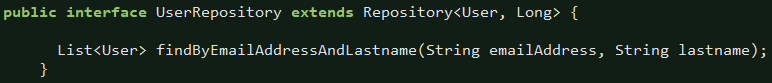
\includegraphics[scale=0.8]{images/repositorySpringData}
	\caption{Exemple de repository}
	\label{fig:repositorySpringData}
\end{figure}

Au cas où le nom de la méthode est trop long ou incommodant dans le programme, ou bien si l’on veut utiliser le nom d’une méthode en modifiant la requête qu’elle doit effectuer, il est possible d’utiliser l’annotation @Query pour changer le nom de la méthode à sa guise. Avant la déclaration de la méthode, cette annotation indiquera la requête que l’on souhaite réaliser lors de l’appel de la fonction.

\begin{figure}
	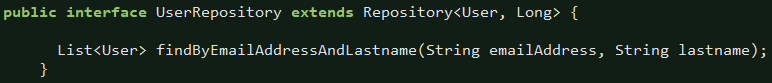
\includegraphics[scale=0.8]{images/repositorySpringData}
	\caption{Exemple de requête spécifié dans un \textit{repository}}
	\label{fig:queryRepository}
\end{figure}

Dans l’exemple de la \autoref{fig:queryRepository}, la requête associée à la méthode \textit{findByEmailAddress()} est modifiée, et est déterminée dans l’annotation @Query. Si la requête effectue des modifications sur les entités, il faut ajouter l’annotation @Modifying et éventuellement si les noms diffèrent, ajouter des annotations @Param pour préciser chaque entité modifiée. 

\begin{figure}
	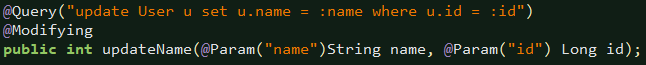
\includegraphics[scale=0.85]{images/queryModifying}
	\caption{Exemple de requête modifiée}
	\label{fig:queryModifying}
\end{figure}

Avec Spring Data JPA, un autre repository est mise à disposition : JPARepository qui regroupe toutes les possibilités des autres repositories et ajoute des méthodes supplémentaires propres à JPA, comme flush() pour le vidage du cache, etc.

\section{Fonctionnement de \textit{Spring Data REST}}

Spring Data Rest est un des modules de Spring Data permettant de faciliter la création de web-services REST. Il constitue une couche supérieure aux dépôts Spring Data et peut exposer les données des dépôts à une application Web. Ainsi, Spring Data nécessite une configuration avec un module de repository comme Spring Data JPA, Spring Data MongoDB, etc.. En général, Spring Data REST n’ajoute pas de fonctionnalités au dépôt de données utilisé. En effet, par définition Spring Data REST doit fonctionner avec n’importe quel projet Spring Data qui utilise un modèle de repository.

La fonctionnalité principale de Spring Data REST est donc d’exporter les ressources des repositories. Ainsi, en configuration standard, un dépôt PersonRepository comme ci-dessous va exposer les ressources à l’URI /persons .

\javacode{public interface PersonRepository extends CrudRepository<Person, Long> \{ \}}

Chaque objet Person sera également exposé selon un modèle d’URI /persons/{id}. Par défaut, les requêtes HTTP effectuées sur le web-service vont interagir avec les méthodes présentes dans CrudRepository de la manière suivante : 

\begin{itemize}
	\item Méthode create -> requête \textbf{POST}
	\item Méthode read -> requête \textbf{GET}
	\item Méthode update -> requête \textbf{PUT}
	\item Méthode delete -> requête \textbf{DELETE}
\end{itemize}

Si l’on souhaite modifier les liens sur lesquelles vont être exportés les ressources, il est possible d’ajouter une annotation @RepositoryRestResource avant la déclaration de l’interface.

\begin{figure}
	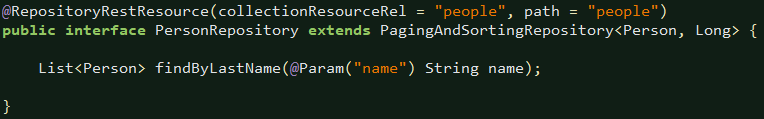
\includegraphics[scale=0.85]{images/repositoryRESTResource}
	\caption{Exposition REST d'un \textit{repository}}
	\label{fig:repositoryRESTResource}
\end{figure}

Dans l’exemple \autoref{fig:repositoryRESTResource}, les objets Person seront exportés sur l’URI /people et plus sur l’URI /persons comme c’était par défaut. L’option collectionResourceRel détermine la valeur à utiliser lors de la génération des liens vers les ressources et l’option path détermine le chemin vers lequel la ressource sera exportée. 

Spring Data Rest ajoute aussi des liens additionnels permettant de naviguer entre les enregistrements. Ces liens sont définis par les méthodes présentes dans le repository de la ressource que l’on recherche. Dans l’exemple précédent, une méthode \textit{findByLastName()} était présente. Ainsi, il est possible de rechercher les personnes par leur nom de famille. Toutes les méthodes de recherche d’un repository sont accessibles avec l’URL /people/search. La syntaxe pour effectuer une recherche sur les noms de famille comme indiquer dans l’exemple serait la suivante : \url{http://localhost:8080/people/search/findByLastName?name=Johnson}. Le résultat de cette recherche donnera toutes les personnes ayant pour nom de famille : Johnson. Les résultats des recherches sont disposés au format JSON. 

\section{Configuration avec \textit{Spring Boot} et \textit{Spring Data JPA}}

L’interfaçage entre Spring Boot, Spring Data JPA et Spring Data REST se fait de façon très simple et automatisé. Spring Boot utilise Spring Data JPA pour créer une implémentation des dépôts et les configurer via une base de données utilisant JPA. Spring Data REST va créer les contrôleurs Spring MVC, les convertisseurs JSON et les autres éléments nécessaires pour obtenir un front-end respectant les règles REST. Spring Boot va ensuite relier les composants du front-end avec les données de JPA de façon automatique. 

Pour lancer un projet utilisant Spring Boot, Spring Data JPA et Spring Data REST, il faut ajouter les deux dépendances spring-boot-starter-data-jpa et spring-boot-starter-data-rest au fichier \textit{pom.xml} comme évoqué dans la \autoref{sec:utilisationMaven}.


\chapter{Angular}

Angular est un framework open-source basé sur le langage TypeScript permettant de réaliser des applications web. Il a été initié par Google en 2016 sous la forme d’un autre framework appelé AngularJS, basé sur JavaScript. Il a été totalement refait par les mêmes équipes pour créer Angular tel qu’on le connaît aujourd’hui. Il est néanmoins nécessaire d’être vigilent lors de la recherche d’informations sur la version d’Angular utilisée, car AngularJS, la version 1 d’Angular, est toujours maintenu et utilisé par certains sites. La version stable d’Angular la plus récente est la version 5, cependant une nouvelle version d’Angular sort environ tous les 6 mois. La version 6 est sortie courant Avril 2018 mais n’est pas encore stable.

L’objectif d’Angular est de faciliter la réalisation d’applications web en automatisant certaines parties et en permettant d’effectuer des animations complexes avec très peu de lignes de code. Les applications Angular sont destinées à fonctionner sur les navigateurs Internet récents (Chrome, Firefox, …) et sont adaptées pour le cross-platform (fonctionner à la fois sur Desktop et sur Mobile). Le framework propose des facilités de développement comme par exemple, la compilation et la génération automatique du code permettant de voir en direct les modifications apportées. La gestion des tests unitaires est également facilitée avec le runner Karma qui permet de voir les résultats de tests directement sur le navigateur et pouvoir modifier à la volée les tests.

\section{Installations nécessaires}

\subsection{Node.js, npm et Angular CLI}

Avant de pouvoir créer un projet, il est nécessaire d’installer plusieurs éléments. Tout d’abord Node.js, une plate-forme logicielle en JavaScript permettant d’utiliser de nombreuses bibliothèques en ligne de commande. Les fichiers d’installation de Node.js se trouvent à l’adresse \url{https://nodejs.org/en/download/}. L’installation de Node.js inclut le gestionnaire de package npm qui permet d’installer des applications Node.js à partir du dépôt npm. L’application se lance depuis une invite de commande, il est possible de vérifier si l’installation s’est faite correctement avec la commande \javacode{npm -v} sur Windows qui indique la version de \textit{npm}. 

Ensuite, la méthode la plus simple pour manipuler un projet Angular est d’utiliser Angular CLI. Il s’agit d’un outil en ligne de commande permettant de créer un projet, d’ajouter des fichiers et d’exécuter des tâches comme l’exécution, le déploiement ou le test d’une application web. L’installation d’Angular CLI se fait avec npm avec la commande : \javacode{npm install -g @angular/cli}.

\subsection{Quelques IDE intéressants pour le développement Angular}

Il existe de nombreux IDE adaptés pour le développement sous Angular. Parmi ces IDE, 3 d’entre eux semblent se démarquer des autres : Angular IDE, WebStorm et l’éditeur en ligne Stackblitz.

\subsubsection{Angular IDE}

Angular IDE est un éditeur gratuit produit par Genuitec optimisé pour le développement Angular. Il a la particularité d’être disponible à la fois en version standalone mais aussi sous forme de plug-in pour Eclipse disponible sur le marketplace. Les téléchargements sont disponibles ici : \url{https://www.genuitec.com/products/angular-ide/}. 

\subsubsection{WebStorm}

WebStorm est l’éditeur faisant parti de la suite produite par Jetbrains avec IntelliJ IDEA, PyCharm et d’autres. C’est un des éditeurs les plus populaires, néanmoins il nécessite l’achat d’une licence commerciale pour l’utilisation. Il apport des fonctionnalités intéressantes comme l’auto-sauvegarde des fichiers, permettant avec Angular de voir en direct les modifications apportées au programme sans avoir à sauvegarder manuellement ses fichiers. 

\subsubsection{Éditeur en ligne: \textit{Stackblitz}}

Stackblitz est un éditeur en ligne adapté à divers types de projets Web. Il comporte les fonctionnalités basiques des IDE locaux intégré directement sur navigateur. Le projet est généré à la volée et on peut voir les modifications en direct sur la même fenêtre. Trois panneaux composent l’interface : un avec l’arborescence, un avec l’éditeur et un autre avec l’émulation du projet. 

Un des avantages de Stackblitz par rapport aux éditeurs locaux est de permettre à plusieurs personnes d’éditer un projet en même temps, à la manière de ce que propose Google Drive. Il est possible de partager le projet entier ou bien uniquement la fenêtre d’affichage. Les projets créés sont Stackblitz peuvent être téléchargés sous forme de dossier compressé. 

\section{Structure d'un projet Angular}

Un projet Angular est basé sur deux concepts : les modules et les composants. La construction d’une application Angular se fait à partir des modules, qui donne un contexte pour la compilation des composants. Un module collecte les différentes fonctions qui lui sont liées pour l’assemblage du projet. Une application Angular est toujours composée d’au moins un module, appelé root module qui assemblent les éléments nécessaires au lancement du programme. 

Les composants définissent les vues de l’application, et une application est constituée d’au moins un composant appelé root component. Chaque composant est définie par au minimum 2 fichier : un fichier HTML qui va définir le modèle d’affichage du composant et un fichier TypeScript avec les données et les fonctions associées à la classe. À ces deux fichiers, on peut en rajouter deux autres qui ne sont pas obligatoires pour le fonctionnement d’un projet : un fichier CSS pour associer un style au template HTML et un autre fichier TypeScript, distingué par une extension .spec.ts, qui définit des tests unitaires.

Les modules et composants de base sont générés lors de la création du projet et donne une arborescence comme on peut le voir sur la \autoref{fig:arborescenceAngular} dans le dossier /src.

\begin{figure}
	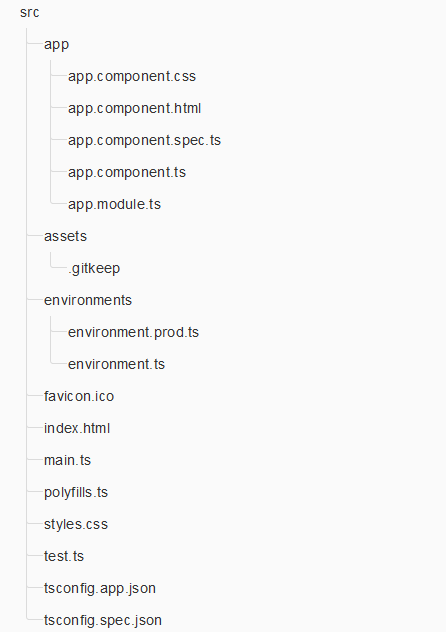
\includegraphics[scale=0.85]{images/arborescenceSrc}
	\caption{Arborescence d'un projet \textit{Angular}}
	\label{fig:arborescenceAngular}
\end{figure}

Ici, le module et le composant par défaut sont disposés dans le dossier app. Les autres fichiers sont détaillés dans la documentation à l’adresse : \url{https://angular.io/guide/quickstart#the-src-folder}.

Le dossier src fait partie des nombreux autres éléments générés à la création d’un projet Angular avec Angular CLI. On retrouve par exemple un dossier node\_module qui comportent tous les modules externes listés dans le fichier package.json présent à la racine du projet. Les autres fichiers sont présentés dans la documentation à l’adresse \url{https://angular.io/guide/quickstart#the-root-folder}.


\section{Gestion des styles: \textit{Bootstrap} et \textit{PrimeNG}}

Il est possible d’appliquer des styles sur les différents composants que l’on souhaite avec les fichiers CSS. Cependant, réaliser un thème cohérent CSS de A à Z est très chronophage. Il existe plusieurs frameworks permettant d’appliquer des thèmes et de réaliser des animations responsives de manière très simple. Par défaut, un projet Angular dispose d’une feuille de style de base appelée styles.css qui est vide. Il permet d’appliquer des styles sur l’ensemble de l’application. Il est possible de changer la feuille de style par défaut appliquée au projet ou bien d’en ajouter plusieurs dans le fichier \textit{.angular-cli.json} au niveau de l’option \textit{styles}.

\begin{figure}
	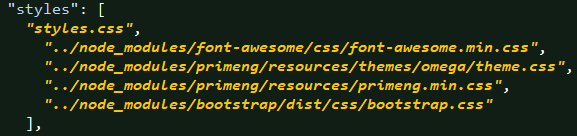
\includegraphics[scale=0.85]{images/styles_angular-cli}
	\caption{Sélection des styles en Angular}
	\label{fig:stylesAngular}
\end{figure}

Parmi les nombreux frameworks existants, en voici deux parmi les plus populaires pour le développement Web actuellement : Bootstrap et PrimeNG.

\subsection{\textit{Bootstrap}}

Bootstrap est une bibliothèque gratuite et open-source permettant de concevoir des applications et des sites web. Utilisée sur un projet, elle permet d’ajouter des éléments responsives, comme des boutons, des panneaux dynamiques et bien d’autres facilement. La bibliothèque est compatible avec la majorité des navigateurs internet sur PC de bureau ainsi que sur mobile. Voici un visuel de ce que peut donner une application avec Bootstrap. 

\begin{figure}
	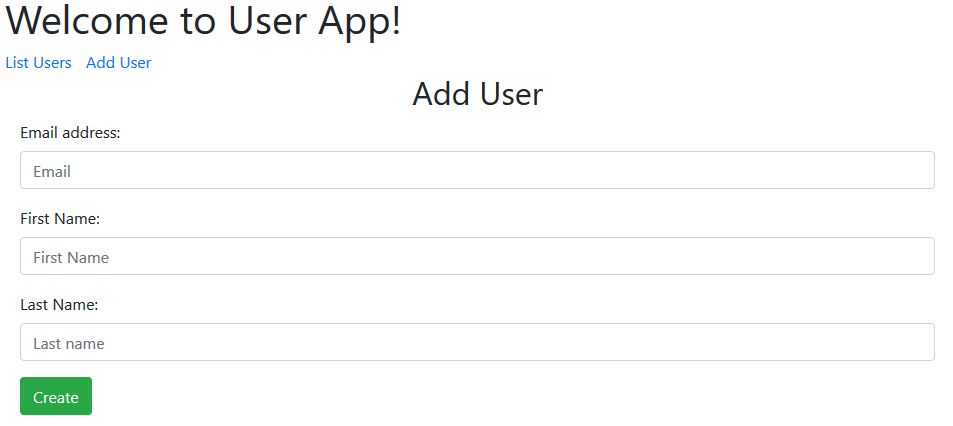
\includegraphics[scale=0.6]{images/bootstrap_exemple}
	\caption{Exemple de page formatée avec \textit{Bootstrap}}
	\label{fig:boostrapExemple}
\end{figure}

Pour utiliser le template Bootstrap avec Angular, il suffit de l’installer en utilisant la commande npm install bootstrap, puis d’ajouter la feuille de style dans le fichier .angular-cli.json comme sur l’image vu auparavant. Ensuite, l’appel des classes se fait via les fichiers HTML relatifs au composant Angular que l’on souhaite voir impacter. La documentation pour pouvoir utiliser pleinement les capacités de Bootstrap se trouve à l’adresse : \url{https://getbootstrap.com/docs/4.1/getting-started/introduction/}.

\subsection{\textit{PrimeNG}}

PrimeNG est une bibliothèque adaptée pour Angular permettant d’ajouter toute sorte de composants et de widgets pour les applications Web. PrimeNG est gratuit, open-source et peut être utilisé de façon complémentaire à Bootstrap. Parmi les composants disponibles, il y a divers types de boutons, de graphiques, de panneaux, compatibles avec différents thèmes. Le site de PrimeNG (\url{https://www.primefaces.org/primeng/#/}) permet de voir directement toutes les possibilités offertes par le framework. 

Pour l’utiliser sur un projet, il faut tout d’abord l’installer avec la commande \javacode{npm install primeng --save}. Une fois installée, de la même manière que pour Bootstrap, il faut ajouter les styles que l’on souhaite dans le fichier \textit{.angular-cli.json}. Par exemple, pour appliquer le thème Omega de PrimeNG, il faut ajouter les styles comme sur la \autoref{fig:stylesPrimeNG}. 

\begin{figure}
	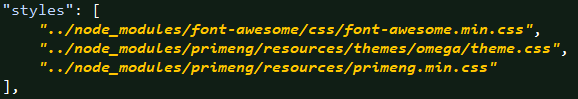
\includegraphics[scale=0.8]{images/styles_primeng}
	\caption{Exemple de styles utilisant \textit{PrimeNG}}
	\label{fig:stylesPrimeNG}
\end{figure}

Ensuite, pour ajouter un module en particulier, par exemple si l’on souhaite ajouter un tableau, il faut importer le module dans le root module de l’application et ensuite, suivre les instructions du site PrimeNG pour voir la balise HTML à utiliser pour ce module. Pour ajouter notre tableau par exemple, le fichier HTML ressemblera à \autoref{fig:primeNGHTML}, avec des balises \textit{p-table} pour représenter le tableau en question.

\begin{figure}
	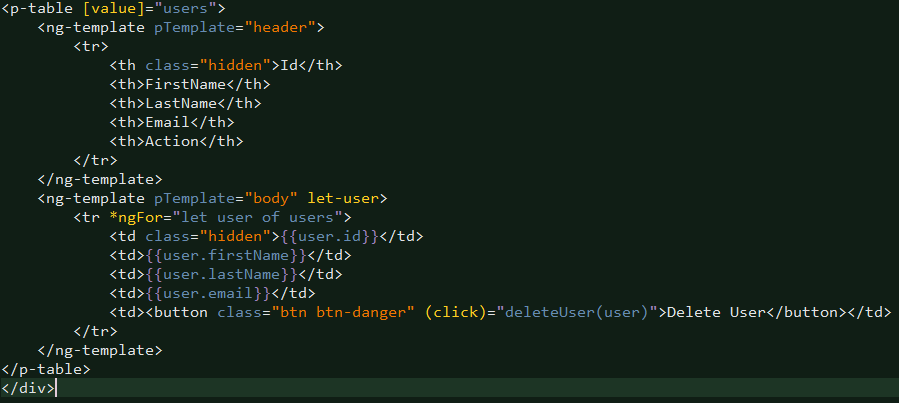
\includegraphics[scale=0.6]{images/primeng_html}
	\caption{Implémentation HTML utilisant \textit{PrimeNG}}
	\label{fig:primeNGHTML}
\end{figure}

\part{Modélisation de l'outil et chiffrage du projet}

Fin Avril jusqu'à début juin

\chapter{Modélisation UML}


\part{Développement}

Juin jusqu'à fin août

\chapter{title}


\chapter{Bilan du stage}


\appendix

\end{document}
